\subsection{Docker Daemon Attack}
If user permissions are incorrectly configured, an unprivileged user can access privileged resources using the Docker daemon. This is shown in \autoref{fig:docker-daemon-attack}.

\begin{figure}[ht]
    \centering
    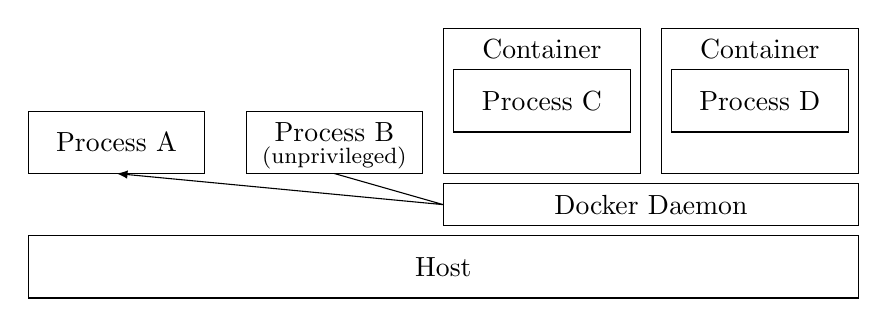
\begin{tikzpicture}[x=0.75pt,y=0.75pt,yscale=-1,xscale=1]
        % Host Rectangle
        \draw (0,100) -- (400,100) -- (400,130) -- (0,130) -- cycle ;
        \draw (200, 115) node {Host};

        %Docker Daemon Rectangle
        \draw (200,75) -- (400,75) -- (400,95) -- (200,95) -- cycle ;
        \draw (300,85) node {Docker Daemon};

        % Process A Rectangle
        \draw (0,40) -- (85,40) -- (85,70) -- (0,70) -- cycle ;
        \draw (42.5,55) node {Process A};

        % Process B Rectangle
        \draw (105,40) -- (190,40) -- (190,70) -- (105,70) -- cycle ;
        \draw (147.5,50) node {Process B};
        \draw (147.5,62.5) node {{\footnotesize (unprivileged)}};

        %Container Process C Rectangle
        \draw (200,0) -- (295,0) -- (295,70) -- (200,70) -- cycle ;
        \draw (247.5,10) node {Container};

        %% Process C Rectangle
        \draw (205,20) -- (290,20) -- (290,50) -- (205,50) -- cycle ;
        \draw (247.5,35) node {Process C};

        %Container Process D Rectangle
        \draw (305,0) -- (400,0) -- (400,70) -- (305,70) -- cycle ;
        \draw (352.5,10) node {Container};

        %% Process D Rectangle
        \draw (310,20) -- (395,20) -- (395,50) -- (310,50) -- cycle ;
        \draw (352.5,35) node {Process D};

        % Line
        \draw [-latex] (147.5,70) -- (200,85) -- (42.5,70);
    \end{tikzpicture}
    \caption{}\label{fig:docker-daemon-attack}
    \medskip
    \small
    An unprivileged process B accessing privileged data (in the image process A) using the Docker daemon.
\end{figure}

The Docker daemon runs as \lstinline{root}. Because Docker has many (powerful) features, this allows any user with permissions to use Docker to practically gain \lstinline{root} privileges. This is why the Docker documentation explicitly states ``only trusted users should be allowed to control your Docker daemon''\footnote{\url{https://docs.docker.com/engine/security/security/}}.

\hfill

A real life example of the impact of incorrectly configured Docker permissions happened a few years back with one of the courses in the Computing Science curriculum (of the Radboud). A teacher wanted to teach students about containerization and modern software development. He asked the IT department to install Docker on all student workstations and add all the students in the course to \lstinline{docker} group (giving them full permissions to run Docker). This gave every student the equivalent of \lstinline{root} rights on every workstation.
